\documentclass{article}

\usepackage[inkscapeformat=png]{svg}
\usepackage{relsize}
\usepackage{adjustbox}
\usepackage{titlesec}
\usepackage{amsmath,amsfonts,amssymb}
\usepackage{mathtools}
\usepackage{enumitem}
\usepackage{listings}
\usepackage{float}
\usepackage[utf8]{inputenc}
\usepackage{xcolor}
\usepackage{graphicx}
\usepackage{subcaption}
\usepackage{tikz}
\usepackage{textcomp}
\usepackage{cite}
\usepackage{apacite}
% \usepackage{hyperref}

\usetikzlibrary{quotes,angles}

\definecolor{codegreen}{rgb}{0,0.6,0}
\definecolor{codegray}{rgb}{0.5,0.5,0.5}
\definecolor{codepurple}{rgb}{0.58,0,0.82}
\definecolor{backcolour}{rgb}{0.95,0.95,0.92}

\newcommand{\md}{~\mathrm d}
\newcommand{\Md}{\mathrm d}
\newcommand{\blankpage}{
    \newpage
    \
    \newpage
}

\lstdefinestyle{mystyle}{
    backgroundcolor=\color{backcolour},   
    basicstyle=\ttfamily\footnotesize,
    breakatwhitespace=false,
    breaklines=true,
    captionpos=b,
    keepspaces=true,
    numbers=left,
    numbersep=5pt,
    showspaces=false,
    showstringspaces=false,
    showtabs=false,
    tabsize=2
}

\graphicspath{ {./assets} }

\bibliographystyle{apacite}

\lstset{style=mystyle}

\author{William B. Sørensen}
\title{MST125 TMA02}
\begin{document}
\maketitle
\tableofcontents

\newpage
\section{Question 1}
\subsection{A}
\subsubsection{i}

\begin{align*}
    g(x, y) &= (7x, 3y) \\
            &= (7x + 0y, 0x + 3y) \\
            &= \begin{bmatrix}
                7 & 0 \\
                0 & 3
               \end{bmatrix}
               \begin{bmatrix}
                   x\\ y
               \end{bmatrix}
\end{align*}

Its type is a $(7,3)$-scaling.

\blankpage
\subsubsection{ii}

\begin{align*}
    h(x, y) &= (x + 3y, y) \\
            &= (x + 3y, 0x + y) \\
            &= \begin{bmatrix}
                1 & 3 \\
                0 & 1
               \end{bmatrix}
               \begin{bmatrix}
                   x\\ y
               \end{bmatrix}
\end{align*}

A horizontal sheer with factor 3

\blankpage
\subsubsection{iii}

\begin{align*}
    k(x, y) &= (y, x) \\
            &= (0x + 1y, 1x + 0y) \\
            &= \begin{bmatrix}
                0 & 1 \\
                1 & 0
               \end{bmatrix}
               \begin{bmatrix}
                   x\\ y
               \end{bmatrix}
\end{align*}

Reflection through line of angle $\frac \pi 4$; reflection through $x=y$.

\blankpage
\subsection{b}

The composite of the operations $k \circ h \circ g$ can be defined as the following matrix product:

\begin{align*}
    (k \circ h \circ g)(\mathbf x) &= k(h(g(\mathbf x))) \\
                                   &= k(h(\mathbf{Gx}))  \\
                                   &= k(\mathbf{HGx})    \\
                                   &= \mathbf{KHGx}
\end{align*}

\begin{align*}
    \mathbf {KHG} = 
           \begin{bmatrix} 0 & 1 \\ 1 & 0 \end{bmatrix}
           \begin{bmatrix} 1 & 3 \\ 0 & 1 \end{bmatrix}
           \begin{bmatrix} 7 & 0 \\ 0 & 3 \end{bmatrix}
        &= \begin{pmatrix}
           \begin{bmatrix} 0 & 1 \\ 1 & 0 \end{bmatrix}
           \begin{bmatrix} 1 & 0 \\ 3 & 1 \end{bmatrix}
           \end{pmatrix}
           \begin{bmatrix} 7 & 0 \\ 0 & 3 \end{bmatrix} \\
        &= \begin{bmatrix} 0 & 1 \\ 1 & 3 \end{bmatrix}
           \begin{bmatrix} 7 & 0 \\ 0 & 3 \end{bmatrix} \\
        &= \begin{bmatrix} 0 & 3 \\ 7 & 9 \end{bmatrix}
\end{align*}

\blankpage
\subsection{c}

$f$ is invertible since

$$\det \mathbf A = 9 \cdot 0 - 7 \cdot 3 = -21 \ne 0$$

Its inverse is

\begin{align*}
    \mathbf A^{-1} &= \frac 1{-21} \begin{bmatrix} 9 & -3 \\ -7 & 0 \end{bmatrix} \\
    &= \begin{bmatrix} -\frac37 & \frac17 \\ \frac13 & 0 \end{bmatrix} \\
    f^{-1}(\mathbf x) &= \mathbf A^{-1}\mathbf x
\end{align*}

\blankpage
\subsection{d}

We start by finding the complement to $\begin{bmatrix} x & y\end{bmatrix}^\top$.

\begin{align*}
    \begin{bmatrix} -\frac37 & \frac17 \\ \frac13 & 0 \end{bmatrix}\begin{bmatrix} x \\ y\end{bmatrix} &= 
    \begin{bmatrix}
        \frac 17 y - \frac 37 x \\
        \frac 13 x
    \end{bmatrix}
\end{align*}

Using this we can substitute the original variables $x,y$ with their complements. Doing this we get the following equation for the mapped unit circle:

\begin{align*}
    \Big( \frac 17 y - \frac 37 x \Big)^2 + \Big( \frac 13 x \Big)^2 &= 1 \\
    \frac {130}{7^2 \cdot 3^2} x^2 - \frac 6{7^2} xy + \frac 1{7^2} y^2 &= 1 \\
    \frac {130}{3^2} x^2 - 6 xy + y^2 &= 49 \\
\end{align*}
\begin{align*}
    a &= \frac {130}{9} &
    b &= -6 &
    c &= 1 &
    d &= 49
\end{align*}

\blankpage
\subsection{e}

We know the area of the unit circle is $1^2\pi = \pi$. A matrix scales areas by the absolute value of the determinant. This means the area must be

$$|\det A| \pi = |-21|\pi = 21\pi$$

\blankpage
\section{2}
\subsection{a}
\subsubsection{i}

Using the fact that a matrix by definition maps the following:

\begin{align*}
    \begin{bmatrix}
        a & b \\ c & d
    \end{bmatrix}
    \begin{bmatrix} 1 \\ 0 \end{bmatrix}
    & =
    \begin{bmatrix} a \\ c \end{bmatrix}
    \\
    \begin{bmatrix}
        a & b \\ c & d
    \end{bmatrix}
    \begin{bmatrix} 0 \\ 1 \end{bmatrix}
    & =
    \begin{bmatrix} b \\ d \end{bmatrix}
    \\
    \begin{bmatrix}
        a & b \\ c & d
    \end{bmatrix}
    \begin{bmatrix} 0 \\ 0 \end{bmatrix}
    & =
    \begin{bmatrix} 0 \\ 0 \end{bmatrix}
\end{align*}

Using this we know that $\mathbf a = \begin{bmatrix} -5 & -6\end{bmatrix}^\top$ since:

\begin{align*}
    f\begin{pmatrix}
        \begin{bmatrix} 0 \\ 0\end{bmatrix}
    \end{pmatrix} &= \mathbf{A\begin{bmatrix} 0 \\ 0\end{bmatrix} + a} \\
                  &= \mathbf{\begin{bmatrix} 0 \\ 0\end{bmatrix} + a} \\
                  &= \mathbf{a} \\
                  &= \begin{bmatrix} -5 \\ -6\end{bmatrix}
\end{align*}

Then following this we get

\begin{align*}
    f\begin{pmatrix} \begin{bmatrix} 1 \\ 0\end{bmatrix} \end{pmatrix}
        &= \mathbf{A\begin{bmatrix} 1 \\ 0\end{bmatrix} + a} &
    f\begin{pmatrix} \begin{bmatrix} 0 \\ 1\end{bmatrix} \end{pmatrix}
        &= \mathbf{A\begin{bmatrix} 0 \\ 1\end{bmatrix} + a} \\
        &= \begin{bmatrix} a \\ c\end{bmatrix} + \mathbf a &
        &= \begin{bmatrix} b \\ d\end{bmatrix} + \mathbf a \\
    \begin{bmatrix} -6 \\ -6\end{bmatrix}
        &= \begin{bmatrix} a \\ c\end{bmatrix} + \begin{bmatrix} -5 \\ -6\end{bmatrix} &
    \begin{bmatrix} -5 \\ -7\end{bmatrix}
        &= \begin{bmatrix} b \\ d\end{bmatrix} + \begin{bmatrix} -5 \\ -6\end{bmatrix} \\
    \begin{bmatrix} -6 \\ -6\end{bmatrix} - \begin{bmatrix} -5 \\ -6\end{bmatrix}
        &= \begin{bmatrix} a \\ c\end{bmatrix} &
    \begin{bmatrix} -5 \\ -7\end{bmatrix} - \begin{bmatrix} -5 \\ -6\end{bmatrix}
        &= \begin{bmatrix} b \\ d\end{bmatrix} \\
    \begin{bmatrix} -6 \\ -6\end{bmatrix} + \begin{bmatrix} 5 \\ 6\end{bmatrix}
        &= \begin{bmatrix} a \\ c\end{bmatrix} &
    \begin{bmatrix} -5 \\ -7\end{bmatrix} + \begin{bmatrix} 5 \\ 6\end{bmatrix}
        &= \begin{bmatrix} b \\ d\end{bmatrix} \\
    \begin{bmatrix} -1 \\ 0\end{bmatrix}
        &= \begin{bmatrix} a \\ c\end{bmatrix} &
    \begin{bmatrix} 0 \\ -1\end{bmatrix}
        &= \begin{bmatrix} b \\ d\end{bmatrix} \\
\end{align*}

This results in the function:
\begin{align*}
    f(\mathbf x) &= \begin{bmatrix}
        -1 & 0 \\ 0 & -1
        \end{bmatrix}\mathbf x + \begin{bmatrix} -5 \\ -6\end{bmatrix} \\
    &= \begin{bmatrix}
        -1 & 0 \\ 0 & -1
        \end{bmatrix}\mathbf x - \begin{bmatrix} 5 \\ 6\end{bmatrix} \\
   &= -\mathbf {Ix} - \begin{bmatrix} 5 \\ 6\end{bmatrix} \\
   &= -\mathbf x - \begin{bmatrix} 5 \\ 6\end{bmatrix}
\end{align*}
\begin{center} NOTE: $\mathbf I$ is the identity matrix \end{center}

being comprised of $(-1)$-dilation followed by a translation $\begin{bmatrix} 5 & 6\end{bmatrix}^\top$.

So in $f(\mathbf x) = \mathbf{Ax + a}$ we get:

\begin{align*}
    \mathbf A &= \begin{bmatrix} -1 & 0 \\ 0 &-1 \end{bmatrix} &
    \mathbf a &= \begin{bmatrix} 5 \\ 6\end{bmatrix}
\end{align*}

\blankpage
\subsubsection{ii}

To find fixed points we use the following equation $\mathbf a = f(\mathbf a)$.

\begin{align*}
    \begin{bmatrix}a\\b\end{bmatrix} &=
        -\begin{bmatrix}a\\b\end{bmatrix}
        - \begin{bmatrix} 5 \\ 6\end{bmatrix} \\
    2\begin{bmatrix}a\\b\end{bmatrix} &=
        - \begin{bmatrix} 5 \\ 6\end{bmatrix} \\
    \begin{bmatrix}a\\b\end{bmatrix} &=
        - \begin{bmatrix} \frac 52 \\ 3\end{bmatrix} \\
\end{align*}

The only fixed point of the function $f$ is the vector $\begin{bmatrix} \frac 52 & 3 \end{bmatrix}^\top$. To test this we do the following:

\begin{align}
    f \begin{pmatrix}
        - \begin{bmatrix} \frac 52 \\ 3\end{bmatrix} \\
    \end{pmatrix} &= 
    \begin{bmatrix} \frac 52 \\ 3\end{bmatrix} - \begin{bmatrix} 5 \\ 6\end{bmatrix} \\
        &= -\begin{bmatrix} \frac 52 \\ 3\end{bmatrix}
\end{align}

The function is also a glide-reflection.

\blankpage
\subsection{b}

Finding $h$ is trivial, the matrix is $\mathbf I$ and the vector transform is logical to find

\begin{align*}
    h(\mathbf x)      &= \mathbf {Ix} - \begin{bmatrix} 8 \\ 0\end{bmatrix} &
    h^{-1}(\mathbf x) &= \mathbf {Ix} + \begin{bmatrix} 8 \\ 0\end{bmatrix}
\end{align*}

We use the definition a reflection along the line with angle $\alpha = -\frac\pi4$

\begin{align*}
    \mathbf B
    &= \begin{bmatrix}
        \cos 2\alpha & \sin 2 \alpha \\
        \sin 2\alpha & -\cos 2 \alpha \\
       \end{bmatrix} \\
    &= \begin{bmatrix}
        0 & -1\\
        -1 & 0
       \end{bmatrix} \\
\end{align*}

$$r(\mathbf x) = \mathbf {Bx}$$

Then finally

\begin{align*}
    (r \circ h)(\mathbf x)
        &= \mathbf {Bx} + \mathbf B\begin{bmatrix} -8 \\ 0\end{bmatrix} \\
        &= \mathbf {Bx} + \begin{bmatrix} 0 \\ 8\end{bmatrix} \\
    (h^{-1} \circ r \circ h)(\mathbf x)
        &= \mathbf {Bx} + \begin{bmatrix} 0 \\ 8\end{bmatrix} + \begin{bmatrix} 8 \\ 0\end{bmatrix}\\
        &= \mathbf {Bx} + \begin{bmatrix} 8 \\ 8\end{bmatrix} & 
    \mathbf b &= \begin{bmatrix} 8 \\ 8\end{bmatrix} \\
        &= \mathbf {Bx + b} \\
        &= \begin{bmatrix}
            0 & -1 \\
            -1 & 0
        \end{bmatrix}\mathbf x + \begin{bmatrix} 8 \\ 8\end{bmatrix}
\end{align*}

\blankpage
\section{3}
\subsection{a}

First conduct the polynomial div.

$$
\begin{matrix}
    3 x^3 & - 4 x^2 & - 21 x & - 24 \\
    \hline 
          & x ^ 2   & - 3  x & - 4 \\
    -3x^3 & + 9 x^2 & + 12 x \\
    \hline
          & 5   x^2 & - 9 x & - 24 \\
          & -5  x^2 & +15 x & + 20 \\
    \hline
          &         &  6 x & - 4
\end{matrix} ~~ = 3x + 5 + \frac{6 x - 4}{x ^ 2 - 3  x - 4}
$$
\begin{center}
    NOTE: Ugly formatting could be avoided using Array environment which I do not know how to use.
\end{center}

Following this we factorize the denominator

\begin{align*}
    v &= \frac{-3 \pm \sqrt{9 + 16}}{2} \\
    v &= \frac{-3 \pm 5}2 \\
    v &\in \{ -1,4 \}
\end{align*}
$$\therefore$$
$$x^2 - 3x - 4 = \prod_{z \in v}(x - z) = (x + 1) (x - 4)$$

Following this we can use the Heaviside cover up method.

\begin{align*}
    \frac{6 x - 4}{(x + 1) (x - 4)} &= \frac A {x + 1} + \frac B {x - 4}
    & A &= \frac{6 \cdot (-1) - 4}{-1 - 4} = \frac{-10}{-5} = 2 \\
        &= \frac 2 {x + 1} + \frac 4 {x - 4}
        & B &= \frac{6 \cdot 4 - 4}{4 + 1} = \frac{20}5 = 4
\end{align*}

Finally we get the partial fraction decomposition to be

$$\frac{3 x^3 - 4 x^2 - 21 x - 24}{x ^ 2 - 3  x - 4} = 3x + 5 + \frac2{x+1}+\frac4{x-4}$$

\blankpage
\subsection{b}

\begin{figure}[H]
    \centering
    \adjustbox{trim=0cm 0cm 0cm 0cm}{\includesvg[width=.9\textwidth]{output}}
    \label{fig:maximaout}
    \caption{Maxima output generated by the print function and selecting SVG}
\end{figure}

\blankpage
\subsection{c}

Let us first declare the integration methods we plan to apply:

\begin{align*}
    \int A(x) + B(x) \md x &= \int A(x) \md x + \int B(x) \md x \\
    \int A(ax + b) \md x   &= \frac 1a \int A(u) \md u \\
    \int k A(x) \md x      &= k \int A(x) \md x \\
    \int x^k \md x         &= \frac 1 {k+1} x^{k+1} + C & k \in \mathrm Z/-1 \\
    \int x^{-1} \md x      &= \ln {|x|} + C
\end{align*}

Then we conduct the integral

\begin{align*}
    \int\frac{3 x^3 - 4 x^2 - 21 x - 24}{x ^ 2 - 3  x - 4} \md x
         &= \int3x + 5 + \frac2{x+1} + \frac4{x-4} \md x\\
         &= \int3x\md x + \int5\md x + \int \frac2{x+1}\md x + \int\frac4{x-4} \md x
\end{align*}
\begin{align*}
    \int3x\md x &= \frac 32 x^2 + C_0 &
    5\int\md x  &= 5 x + C_1 \\
    \int \frac2{x+1}\md x &= 2 \int \frac1{x+1}\md x &
    \int \frac4{x-4}\md x &= 4 \int \frac1{x-4}\md x \\
                          &= 2 \int \frac1u\md u &
                          &= 4 \int \frac1{u}\md u \\
                          &= 2 \ln {|x+1|} + C_2 &
                          &= 4 \ln {|x+4|} + C_3 \\
\end{align*}

$$
\int\frac{3 x^3 - 4 x^2 - 21 x - 24}{x ^ 2 - 3  x - 4} \md x =
\frac 32 x^2 + 5x + 2 \ln {|x+1|} + 4 \ln {|x+4|} + C
$$

\blankpage
\section{4}
\subsection{a}

Since the denominator would be zero at $x = 3$ then the domain is $x\in\mathbb R /3$ that can also be written $x\in\langle\infty,3\rangle\cup\langle3,\infty\rangle$.

Its $x$-intercept would be found with

\begin{align*}
    0 &= \frac{x^2 + 12}{(x-3)^2} \\
    0 &= x^2 + 12 \\
    x &= \pm 2\sqrt{3}i
\end{align*}

$f$'s $x$-intercepts reside on the complex plane (in this case the imaginary axis).

$f$'s $y$-intercept would be found with

\begin{align*}
    y &= \frac{12}{(-3)^2} \\
    y &= \frac{12}{9} \\
    y &= \frac{4}{3} \\
\end{align*}

$f$'s y intercept is located at $y = \frac 43$

\blankpage
\subsection{b}

\begin{align*}
    f(x) &= \frac{x^2 + 12}{(x-3)^2} \\
    \frac{\Md f}{\Md x} &= ((x^2 + 12)(x-3)^{-2})' \\
                        &= (x^2 + 12)'(x-3)^{-2} + (x^2 + 12){(((x-3)^{-2})}' \\
                        &= 2x(x-3)^{-2} + -2(x^2 + 12)(x-3)^{-3} \\
                        &= 2x(x-3)^{-3}(x-3) + -2(x^2 + 12)(x-3)^{-3} \\
                        &= \frac{2x(x-3) + -2(x^2 + 12)}{(x-3)^3} \\
                        &= \frac{-6x -24}{(x-3)^3}
\end{align*}

\blankpage
\subsection{c}

The stationary points are located at $f'(x)=0$.

\begin{align*}
    \frac{-6x -24}{(x-3)^3} &=  0 \\
    \frac{x + 4}{(x-3)^3}   &=  0 \\
    x + 4                   &=  0 \\
    x                       &= -4 \\
\end{align*}

Then we get $f(-4)$.

\begin{align*}
    f(-4) &= \frac{16 + 12}{(-4-3)^2} \\
          &= \frac{36}{49} \\
\end{align*}

The stationary point is located at $(-4, \frac{36}{49})$

\begin{figure}[H]
    \centering
    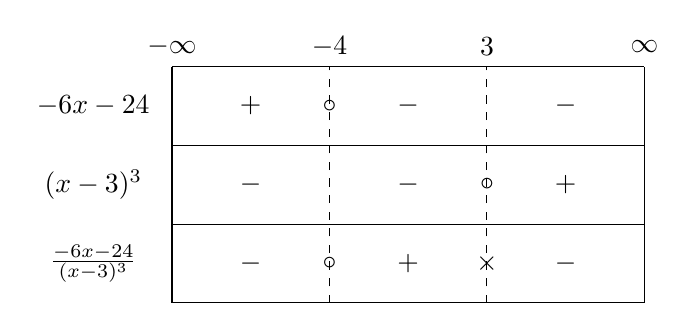
\begin{tikzpicture}
        % box and vertical lines
        \draw (-3, 0) -- ( 3, 0); % Bottom Line
        \draw (-3, 1) -- ( 3, 1); % Center Line
        \draw (-3, 2) -- ( 3, 2); % Center Line
        \draw (-3, 3) -- ( 3, 3); % Top    Line

        \draw (-3, 0) -- (-3, 3); % Left   Line
        \draw [dashed](-1, 0) -- (-1, 3); % MLeft  Line
        \draw [dashed]( 1, 0) -- ( 1, 3); % MRight Line
        \draw ( 3, 0) -- ( 3, 3); % Right  Line

        % Bottom row
        \node (A) at (-2, 0.5) {$-$};
        \node (A) at (-1, 0.5) {$\circ$};
        \node (A) at ( 0, 0.5) {$+$};
        \node (A) at ( 1, 0.5) {$\times$};
        \node (A) at ( 2, 0.5) {$-$};

        % Center row
        \node (A) at (-2, 1.5) {$-$};
        \node (A) at ( 0, 1.5) {$-$};
        \node (A) at ( 1, 1.5) {$\circ$};
        \node (A) at ( 2, 1.5) {$+$};

        % Top row
        \node (A) at (-2, 2.5) {$+$};
        \node (A) at (-1, 2.5) {$\circ$};
        \node (A) at ( 0, 2.5) {$-$};
        \node (A) at ( 2, 2.5) {$-$};

        \node (A) at (-3, 3.25) {$-\infty$};
        \node (A) at ( 3, 3.25) {$ \infty$};
        \node (A) at (-1, 3.25) {$-4$};
        \node (A) at ( 1, 3.25) {$3$};

        \node (A) at (-4, 0.5) {$\frac{-6x - 24}{(x-3)^3}$};
        \node (A) at (-4, 1.5) {$(x-3)^3$};
        \node (A) at (-4, 2.5) {$-6x - 24$};
    \end{tikzpicture}

    \caption{Table of signs for $f$ rendered in Tikz}
    \label{fig:tos4}
\end{figure}

By the definition of increasing and decreasing we can see that $f$ is decreasing in the interval $\langle\infty, -4\rangle \cup \langle 3, \infty \rangle$ and increasing in the range $\langle -4, -3 \rangle$. $f$ is stationary in the point $x=-4$. Since we can see that it is a transition from decreasing to increasing we can conclude it is a local minimum.

\blankpage
\subsection{d}

We begin by conducting a polynomial division.

\begin{align*}
    \frac{x^2 + 12}{(x-3)^2} &= \frac{x^2 + 12}{x^2 - 6 x + 9}
\end{align*}

$$ \begin{matrix}
    x^2  &+& 0 x &+& 12 \\
    \hline
    x^2  &-& 6 x &+& 9 \\
    -x^2 &+& 6 x &-& 9 \\
    \hline
         & & 6 x &+& 3 \\
\end{matrix} ~~ = 1 + \frac{6x + 3}{(x-3)^2}$$

From this we see that

$$ \lim_{x \to \infty} \Big(1+\frac{6x + 3}{(x-3)^2}\Big) = 1 $$

Hence there is a horizontal asymptote $y = 1$. We also have a vertical asymptote at $x = 3$. These will be included in the sketch bellow.

\blankpage
\subsection{e}

We can do a proof by contradiction in this case

\begin{align*}
    x &= 1 & x &= -1 \\
    \hline
    l &= \frac{1^2 + 12}{(1-3)^2} &
    r &= \frac{(-1)^2 + 12}{(-1-3)^2} \\
    l &= \frac{13}{4} &
    r &= \frac{13}{16} \\
\end{align*}

As we can see $r \ne l$ so $f$ is not even and $r \ne -l$ so its not odd either.

% Since we know that

% We can make our lifes slightly easier in the following calculations by using the expantion over the alternative. Also since 1 is an even function one would need a discontinus function at the point $x=0$ to be able to allow the function to be odd which then makes it impossible since we know we do not have a discontinus function in $x=0$.

% Following to test for evenness we can simply view that:

% TODO

\blankpage
\subsection{f}

First compute some values to include in the sketch.

\begin{align*}
f(-6) &= \frac{(-6)^2 + 12}{(-6-3)^2} & 
f(-4) &= \frac{(-4)^2 + 12}{(-4-3)^2} & 
f(-2) &= \frac{(-2)^2 + 12}{(-2-3)^2} \\
     &= 0.59&
     &= 0.57&
     &= 0.64\\
f(2) &= \frac{(2)^2 + 12}{(2-3)^2} &
f(4) &= \frac{(4)^2 + 12}{(4-3)^2} & 
f(6) &= \frac{(6)^2 + 12}{(6-3)^2} \\
     &= 16.0&
     &= 28.0&
     &= 5.33\\
f(5) &= \frac{(5)^2 + 12}{(5-3)^2} &
f(7) &= \frac{(7)^2 + 12}{(7-3)^2} & 
f(8) &= \frac{(8)^2 + 12}{(8-3)^2} \\
     &= 9.25&
     &= 3.812&
     &= 3.04\\
\end{align*}

Finally we include the asymptotic $x=3$ and $y=1$ and the turning point $(-4,0.57)$.

\begin{figure}[H]
    \centering
    \adjustbox{trim=0cm 0cm 0cm 0cm}{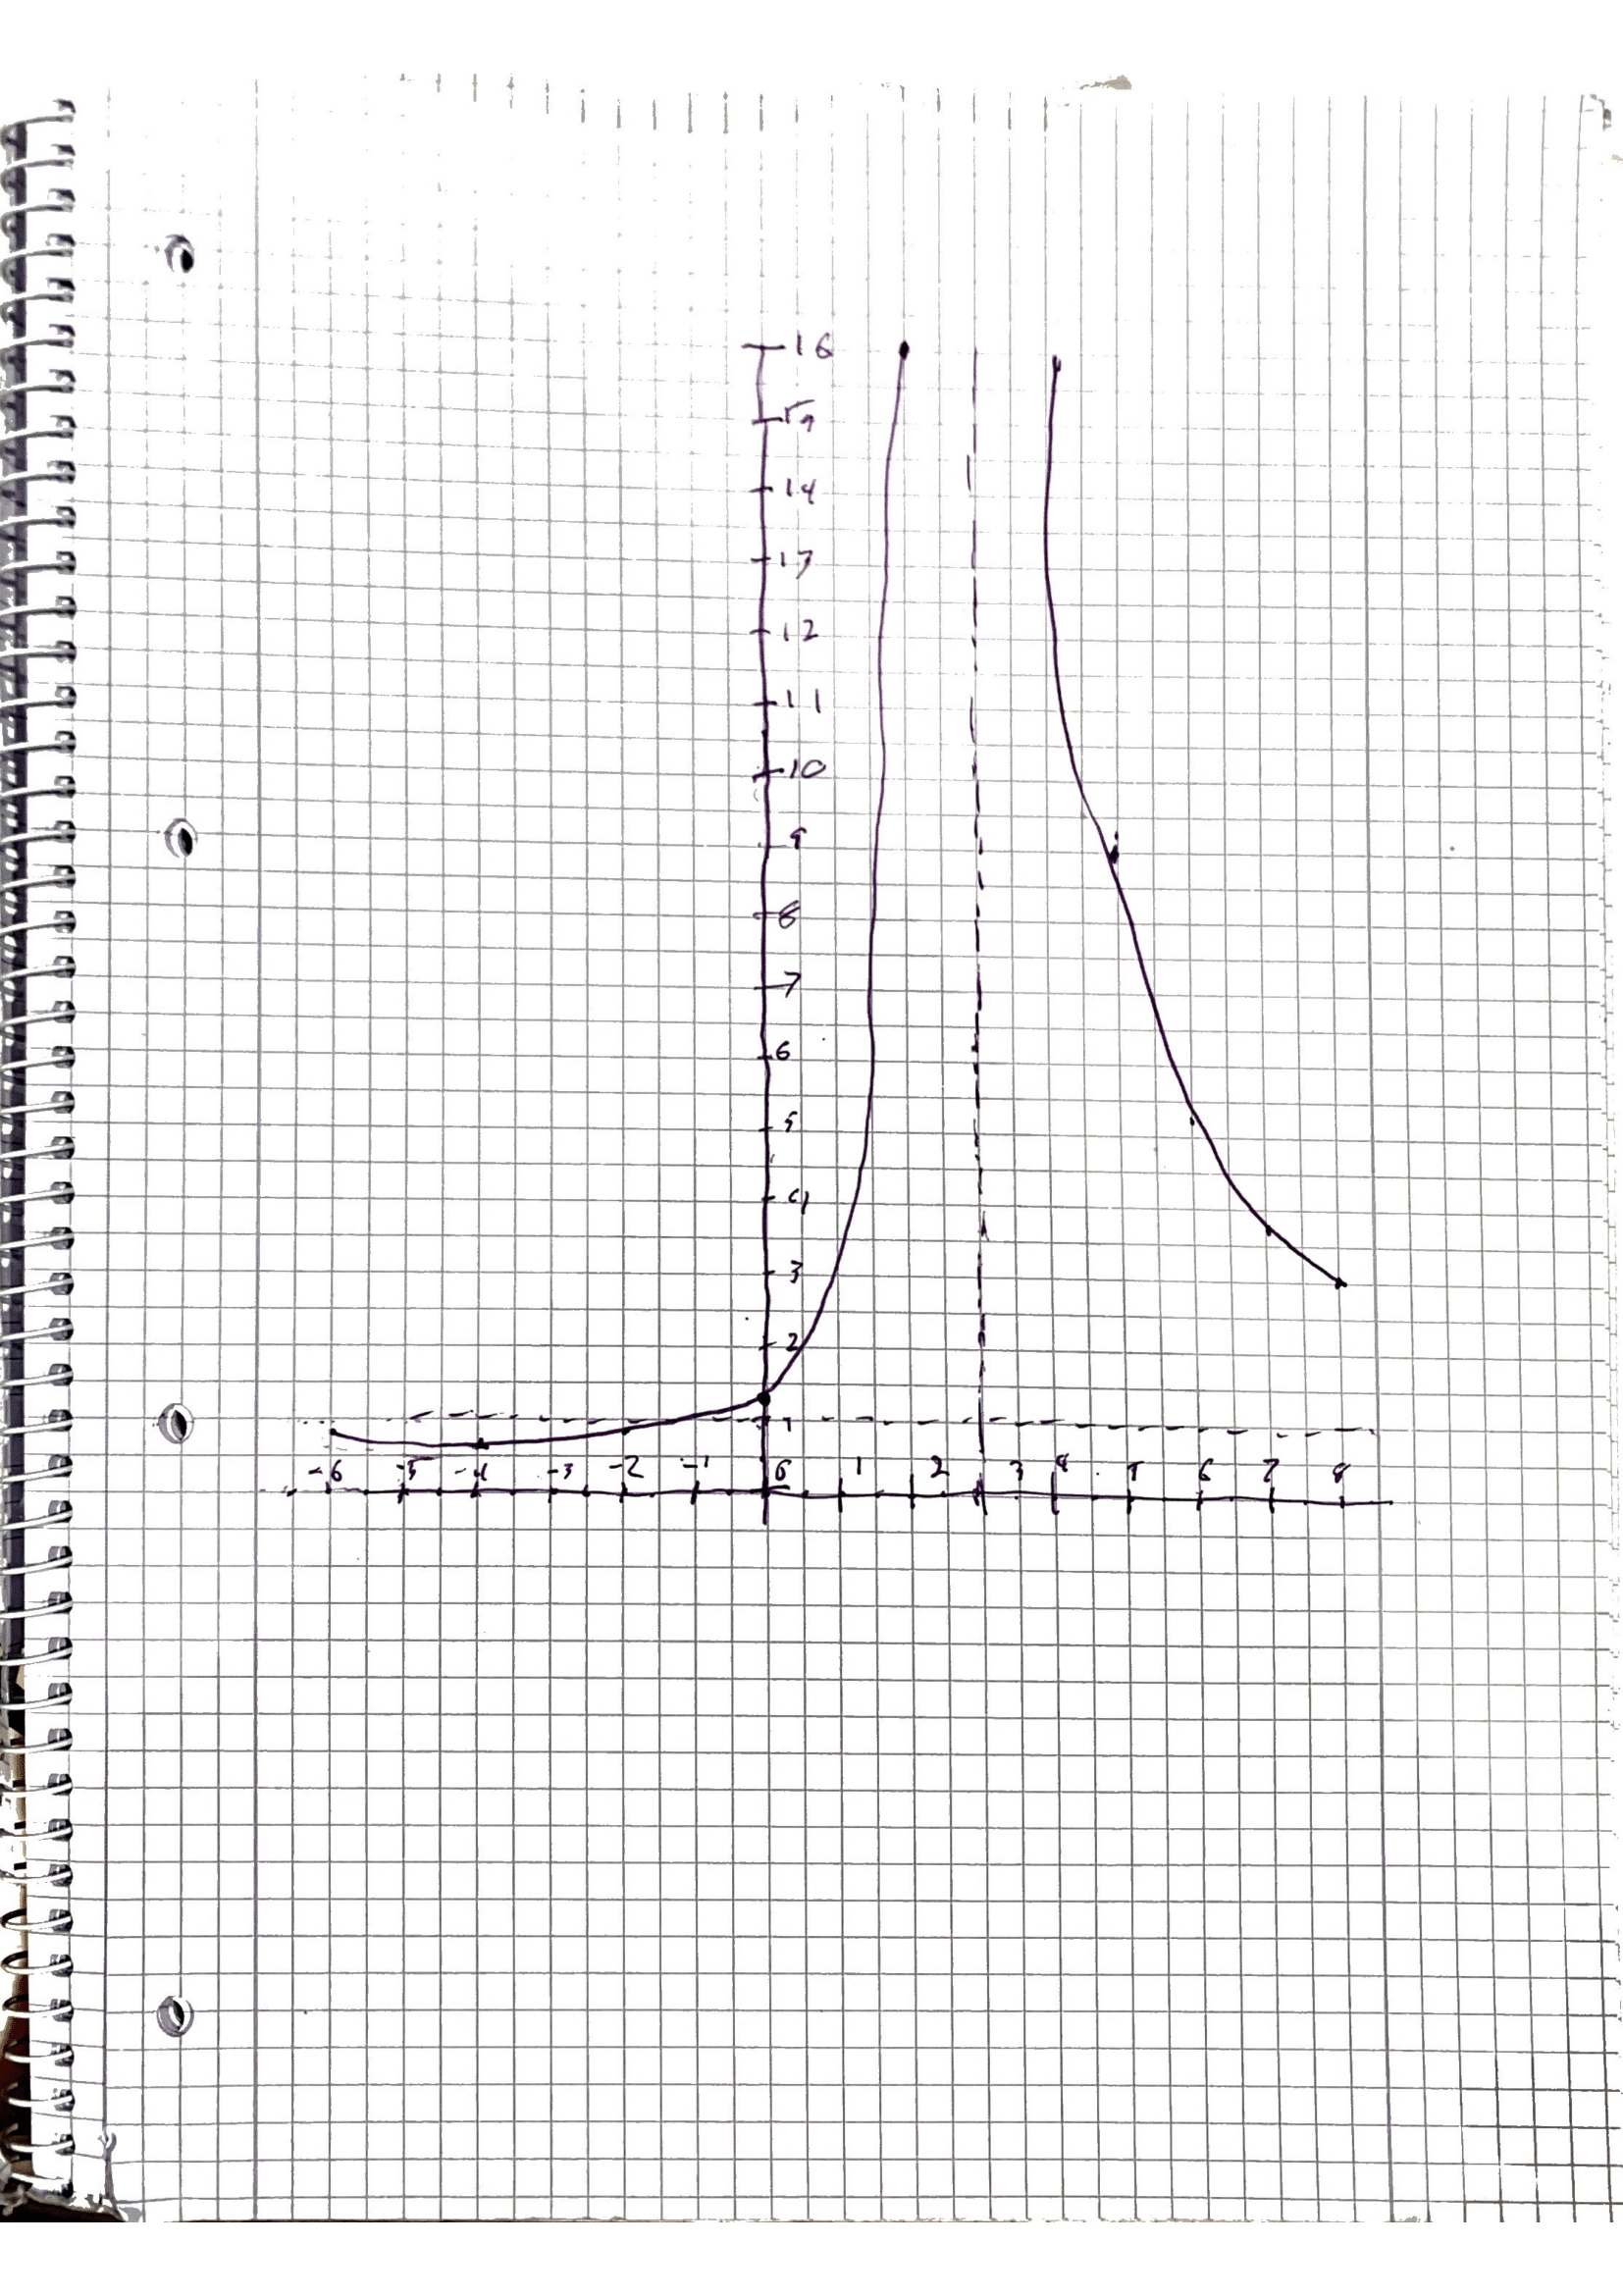
\includegraphics[width=.9\textwidth]{sketch-TMA02.png}}
    \label{fig:sketch}
    \caption{Sketch of graph $f$ scanned from paper}
\end{figure}

% \begin{figure}[H]
%     \centering
%     \begin{tikzpicture}[domain=-15:15,scale=0.25]
%         \draw[very thin,color=lightgray,step=2] (-15.1,-5.1) grid (14.9,20.9);

%         \draw[->] (-15,0) -- (15, 0) node[right] {$x$};
%         \draw[->] (0, -5) -- (0, 22) node[above] {$f(x)$};

%         \draw[dashed] (-15,1) node[left] {$y=1$} -- (15, 1);
%         \draw[dashed] (3, -5) -- (3, 22) node[above right] {$x=3$};

%         \draw[color=blue,yrange=-20:20]
%             plot (\x, {min(20,2+(\x^2 + 12)/((\x-3)^2+.01))})
%             node[right] {$f(x) = \frac{x^2 + 12}{(x-3)^3}$};
%     \end{tikzpicture}
% \end{figure}

\blankpage
\section{5}
\subsection{a}
\subsubsection{i}

For this example we will use the chain rule defined to $(f(u(x)))' = u'(x) f'(u(x))$.

\begin{align*}
    (4^x)' &= (e^{\ln 4 ~ x})' & f(x) = e^x, &~ u(x) = \ln 4 x \\
           &= (f(u(x)))' & f'(x) = e^x,&~ u'(x) = \ln 4 \\
           &= u'(x)f'(u(x)) \\
           &= \ln 4 ~ e^{\ln 4 x} \\
           &= \ln 4~4^x
\end{align*}

\blankpage
\subsubsection{ii}

\begin{align*}
    \int 4^x \sin 4^x \md x &= \frac 1 {\ln 4}\int \sin u \md x \\
                            &= -\frac 1 {\ln 4} \cos 4^x + C
\end{align*}

\blankpage
\subsection{b}

The given trig identity i use in this case is $\cos^2 x = \frac 12 (\cos 2x + 1)$.

\begin{align*}
    \int 3x^2 \cos^2 x^3 \md x &= \int \cos^2 u \md u \\
                               &= \frac12 \int \cos 2u + 1 \md u \\
                               &= \frac14 \int \cos z + 1 \md z \\
                               &= \frac14 (z + \sin z) + C \\
                               &= \frac14 (2u + \sin 2u) + C\\
                               &= \frac14 (2x^3 + \sin 2x^3) + C\\
                               &= \frac12x^3 + \frac14\sin 2x^3 + C\\
\end{align*}

\blankpage
\section{6}
\subsection{a}

The form of the equation is direct integration. This means its of the form:

$$\frac{\Md y}{\Md x} = f(x)$$

The method used to solve this goes as follows:

$$\int\md y = \int f(x)\md x$$

\blankpage
\subsection{b}

\begin{align*}
    \frac{\Md x}{\Md t} &= \frac{e^t}{e^t + 3} \\
    \int\md x &= \int\frac{e^t}{e^t + 3}\md t \\
    x + C_0   &= \int\frac 1 u \md u \\
              &= \ln |u| + C_1 \\
              &= \ln (e^t + 3) + C_1 \\
              &= \ln (e^t + 3) + C_1 \\
    x(t)      &= \ln (e^t + 3) + C
\end{align*}

\begin{center}
    NOTE/TANGENT: This function is actually very similar to the soft-plus activation function which i think is quite cool to see.
\end{center}

\blankpage
\subsection{c}

\begin{align*}
    17 &= \ln (e^0 + 3) + C \\
    17 &= \ln 4 + C \\
    17 - 2\ln 2 &= C \\
\end{align*}

Hence the particular solution for $x(0) = 17$ is:

$$x(t) = \ln(e^t + 3) + 17 - 2 \ln 2$$

\blankpage
\section{7}
\subsection{a}

This differential equation is of the form separable (ordinary) differential equation meaning can be rearranged to the form:

$$\frac{\Md y}{\Md x} = f(y) ~ g(x)$$

These can be solved as the following:

\begin{align*}
    \frac{\Md y}{\Md x} &= f(y) ~ g(x) \\
    \frac{\Md y}{\Md x} \frac1{f(y)} &= g(x) \\
    \int \frac1{f(y)}\md y &= \int g(x) \md x \\
\end{align*}

\blankpage
\subsection{b}

We simply use the method with the function names substituted with the expression and then we get the following:

\begin{align*}
    \frac{\Md y}{\Md t} &= - \frac{y^2}{\sqrt{1 - t^2}} \\
    \int y ^{-2}\md y   &= - \int \frac1{\sqrt{1 - t^2}} \md t \\
    -y^{-1} + c_0       &= - \sin^{-1}t + c_1 \\
    y(t)                &= \frac1{C - \sin^{-1}t}
\end{align*}

\blankpage
\section{8}
\subsection{a}

This differential equation is of the form (ordinary) linear-differential equation and is solved with the following technique.

\begin{align*}
    \frac{\Md y}{\Md x} + f(x)y
        &= g(x) \\
    \Big(\frac{\Md y}{\Md x} + f(x) y\Big) e^{\int f(x) \md x}
        &= g(x) e^{\int f(x) \md x} \\
    \frac{\Md y}{\Md x} e^{\int f(x) \md x} + y ~ f(x) e^{\int f(x) \md x}
        &= g(x) e^{\int f(x) \md x} \\
    \frac{\Md}{\Md x} \big(y ~ e^{\int f(x) \md x}\big)
        &= g(x) e^{\int f(x) \md x} \\
    y ~ e^{\int f(x) \md x}
        &= \int g(x) e^{\int f(x) \md x} \md x \\
    y &= e^{-\int f(x) \md x}
        \int g(x) e^{\int f(x) \md x} \md x \\
\end{align*}

This method proof of integration of linear-differential equations comes from \cite{maths:r2} page 303.

\blankpage
\subsection{b}

\begin{align*}
    \frac{\Md y}{\Md x} - \frac{9 y}x &= x^9 &
        f(x) &= -\frac9x \\
    && \int f(x) \md x &= -9 \ln x + c_0\\
\end{align*}
\begin{align*}
    y(x) &= e^{9 \ln x}\int x^9 e^{-9 \ln x} \md x \\
         &= x^9\int x^9x^{-9} \md x \\
         &= x^9\int \md x \\
         &= x^9(x + c) \\
         &= x^{10} + cx^9 \\
\end{align*}

\blankpage
\section{9}
\subsection{a}

\begin{align*}
    \frac{\Md v}{\Md x} &= \frac kv \\
    \frac{\Md v}{\Md x}v &= k \\
    \int v\md v &= \int k\md x \\
    \frac12v^2 &= kx + c_1
\end{align*}

In case the solution is wanted in explicit form as well

$$v(x) = \sqrt{2kx + c_2}$$

\blankpage
\subsection{b}

We substitute $v=8$ and $x=0$

\begin{align*}
    \frac12v^2 &= kx + c_1 \\
    \frac12(8)^2 &= k0 + c_1 \\
    c_1 &= 32
\end{align*}
We then get this formula
$$ \frac12v^2 = kx + 32 $$

\blankpage
\subsection{c}

We substitute $v=18$ and $x=2$

\begin{align*}
    \frac12v^2 &= kx + 32 \\
    \frac12(18)^2 &= k2 + 32 \\
    \frac12 324 &= k2 + 32 \\
    162 &= k2 + 32 \\
    130 &= k2 \\
    65 &= k \\ \\
    \frac12v^2 &= 65x + 32
\end{align*}

We then get this formula

$$ \frac12v^2 = 65x + 32 $$

\blankpage
\subsection{d}

We use the formula we've seen so far and substitute $v=90$.

\begin{align*}
    \frac12v^2 &= 65x + 32 \\
    \frac{\frac12(90)^2 - 32}{65} &= x \\
    x &= \frac{4018}{65}
\end{align*}

\blankpage
\subsection{e}

\begin{figure}[H]
    \centering
    \adjustbox{trim=0cm 0cm 0cm 0cm}{\includesvg[width=.9\textwidth]{final}}
    \label{fig:maximaouttwo}
    \caption{Maxima output generated by the print function and selecting SVG}
\end{figure}

\blankpage

\bibliography{TMA}

\end{document}
